\chapter*{Appendix C \\ Star-forming/Quiescent Classifications \label{chap:append3}}
\addcontentsline{toa}{appendix}{Appendix C}
\addtocontents{toa}{\addvspace{10pt}}%just to separate the entries in the list

In our parameterization of the observed $\fqcen$ in Eqs.~\ref{eq:fq} and~\ref{eq:fqz0}, 
we derive the best-fit values for the parameters $A_0$ and $A_1$ by fitting 
$\fqcen$ measured in the SDSS DR7 group catalog. The SDSS DR7 group catalog 
$\fqcen$ is derived using a $\mathrm{SFR} - \mathcal{M}_*$ cut 
specified in Eq.~\ref{eq:sfr_cut}. For $\alpha(\mathcal{M}_*)$, the 
parameter that dictates the $\fqcen$ redshift dependence, however, 
the best-fit value is derived from fitting \cite{Tinker:2013aa} 
$\fqcen$ measurements of the COSMOS survey. These $\fqcen$ measurements 
use $(NUV - R) - (R - J)$ color-color cuts described in 
\cite{Bundy:2010aa} for the star-forming/quiescent classification. 
In this section, we demonstrate the consistency between the SDSS 
DR7 group catalog $\fqcen$, using a $\mathrm{SFR} - \mathcal{M}_*$ 
cut, and the \cite{Tinker:2013aa} $\fqcen$, using a $(NUV - R) - (R - J)$ 
color-color cut.

For the galaxies in our SDSS DR7 group catalog, we construct a catalog
with UV, optical, and infrared photometry. For UV and optical, 
we obtain GALEX and SDSS photometry from the NASA-Sloan Atlas\footnote{http://www.nsatlas.org/}.
For infrared, we use photometry from the 2MASS all-sky map~\citep{Cutri:2000aa}. 
We then determine the $FUV, NUV$, $u, g, r, i, z$, $J, H, K_s$ 
band $K$-corrections and absolute magnitudes for the galaxies 
using $\mathtt{K-correct}$\footnote{http://howdy.physics.nyu.edu/index.php/Kcorrect}~\citep[v4.2][]{Blanton:2007aa}. 

Using these absolute magntidues, in Figure~\ref{fig:NUV_R_J}, we 
plot $(NUV-R) - (R-J)$ color-color relation for the SDSS DR7 group 
catalog (black). We highlight the galaxies in the sample that are 
classified as quiescent using the $\mathrm{SFR} - \mathcal{M}_*$
cut in orange. Furthermore, we plot the color-color cuts from 
\cite{Bundy:2010aa} (blue dash-dotted and red dashed lines). 
Galaxies that lie above both color-color cuts, are classified as 
quiescent in the $(NUV-R) - (R-J)$ classification. 

The horizontal color-color cut (blue dash-dotted) is evaluated
using the \cite{Bundy:2010aa} parameterization, at $z \sim 0.0$. The 
diagonal cut (red dashed) in \cite{Bundy:2010aa} is, however, 
parameterized using coefficients determined by inspection of 
redshift bins. Therefore, for the SDSS DR7 group catalog, we 
extrapolate the coefficients from the COSMOS $z \sim 0.3, 0.7$ 
bins. We note that using the coefficients from the lowest COSMOS 
redshift bin ($z \sim 0.3$) instead of extrapolating to $z \sim 0.0$,
does not significantly impact the comparison in this section. 

Comparison of the quiescent galaxies classified with $\mathrm{SFR} - \mathcal{M}_*$ 
with the color-color cuts in Figure~\ref{fig:NUV_R_J} find that
the two classifications are generally consistent. To further 
test whether the different classifications can impact quiescent
fraction parameterization, in Figure~\ref{fig:fq_colorcolor}, we 
compare the the quiescent fractions derived from them for the 
SDSS DR7 group catalog: $\fq^{SFR-\mathcal{M}_*}$ (black) versus 
$\fq^{\rm color}$ (orange). Throughout the mass range of the 
catalog, $\fq^{SFR-\mathcal{M}_*}$ and $\fq^{\rm color}$ are 
consistent with each other. Therefore, the $\fqcen(\mathcal{M}_*, z)$ 
parameterization derived from measurements of SDSS DR 7 group catalog 
and \cite{Tinker:2013aa} (Eq.~\ref{eq:fq}) does {\em not} affect the 
results of this work.

\begin{figure}
\begin{center}
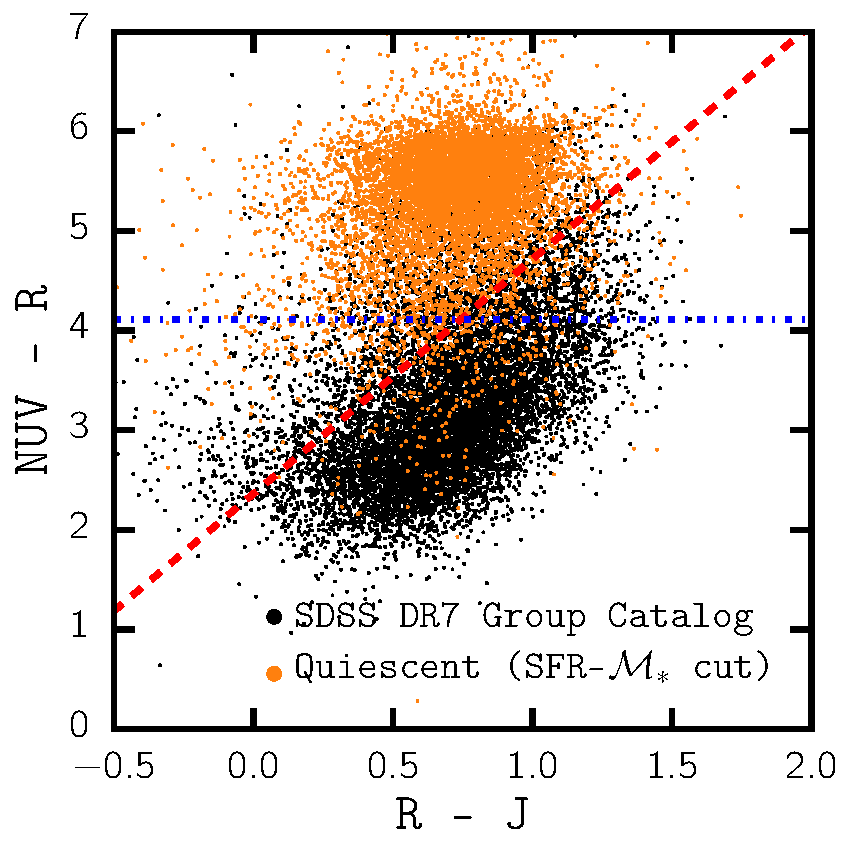
\includegraphics[width=\textwidth]{figs/cenq/nuv_r_j.pdf}
\caption{
The $(NUV - R) - (R - J)$ color-color relation for the
SDSS DR7 group catalog (black) calculated from photometry 
compiled from GALEX, SDSS, and 2MASS (\S~\ref{chap:append2}). 
Galaxies classified as quiescent using the $\mathrm{SFR} - \mathcal{M}_*$ 
cut are highlighted (orange). Furthermore, we plot the color-color 
cuts from \cite{Bundy:2010aa} that describe the classification
of star-forming/quiescent galaxies in \cite{Tinker:2013aa}. 
We note that the quiescent galaxies classified using the 
$\mathrm{SFR} - \mathcal{M}_*$ cut are generally consistent with 
the \cite{Bundy:2010aa} color-color cuts. 
}
\label{fig:NUV_R_J}
\end{center}
\end{figure}

\begin{figure}
\begin{center}
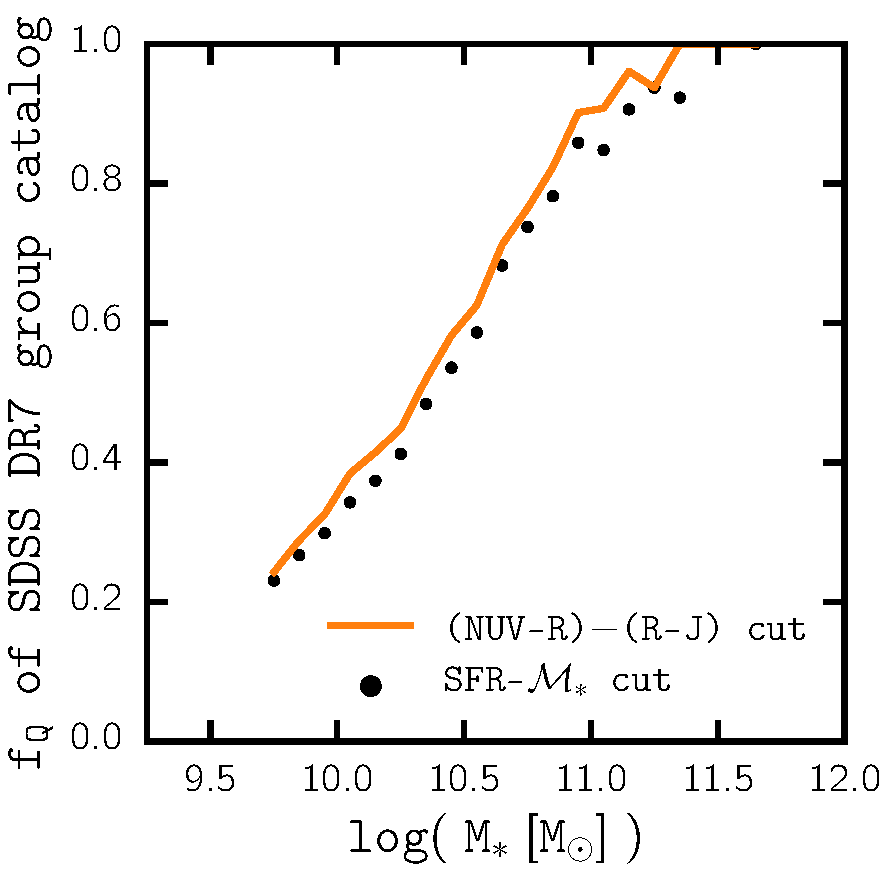
\includegraphics[width=\textwidth]{figs/cenq/fq_colorcolor.pdf}
\caption{Comparison of the SDSS DR7 group catalog $\fq(\mathcal{M}_*)$ 
measured using the $\mathrm{SFR} - \mathcal{M}_*$ versus the 
$(NUV - R) - (R - J)$ color-color classifications. The $\fq$s 
measured using the two different classification methods are
consistent with each other. This consistency illustrates that 
the $\fqcen(\mathcal{M}_*, z)$ parameterization derived from 
measurements of SDSS DR 7 group catalog and \cite{Tinker:2013aa} 
does {\em not} affect the results of this work.}
\label{fig:fq_colorcolor}
\end{center}
\end{figure}
